\section{Implementation Characteristics}
In order to avoid unwanted divergencies, a sc lattice with equal distance between each particle pair is implemented as initial state.
Each implementation requires to choose parameters such that the outcome is plausible.
For an estimation which setting is best, a correlation analysis is sufficient.
This will be explained for the Monte-Carlo algorithm in detail and in short for the Molecular Dynamics simulation.\medskip\\
To access a good amount of states, the steps must show ergodicity.
For this purpose, the step vector $\delta \bm r$ is a uniformly distributed vector on a sphere with norm $\left|\delta\bm r\right| = \epsilon$ per construction\footnote{Uniformly distributed $u=\cos(\theta)$ and $v=\phi$, the resulting vector via spherical coordinates.}.
% The mean movement of each particle now vanishes in equilibrium states.
The reason for choosing an acceptance ratio of \SI{60}{\percent} lies within the correlation of quantity measurements.
Taken the energy, for a $4\times10^4$ sample after $10^5$ MC-Steps, the correlation length differs according to the acceptance ratio (see Fig.~\ref{fig:MCCorrSeries}).
\begin{figure}[ht]
	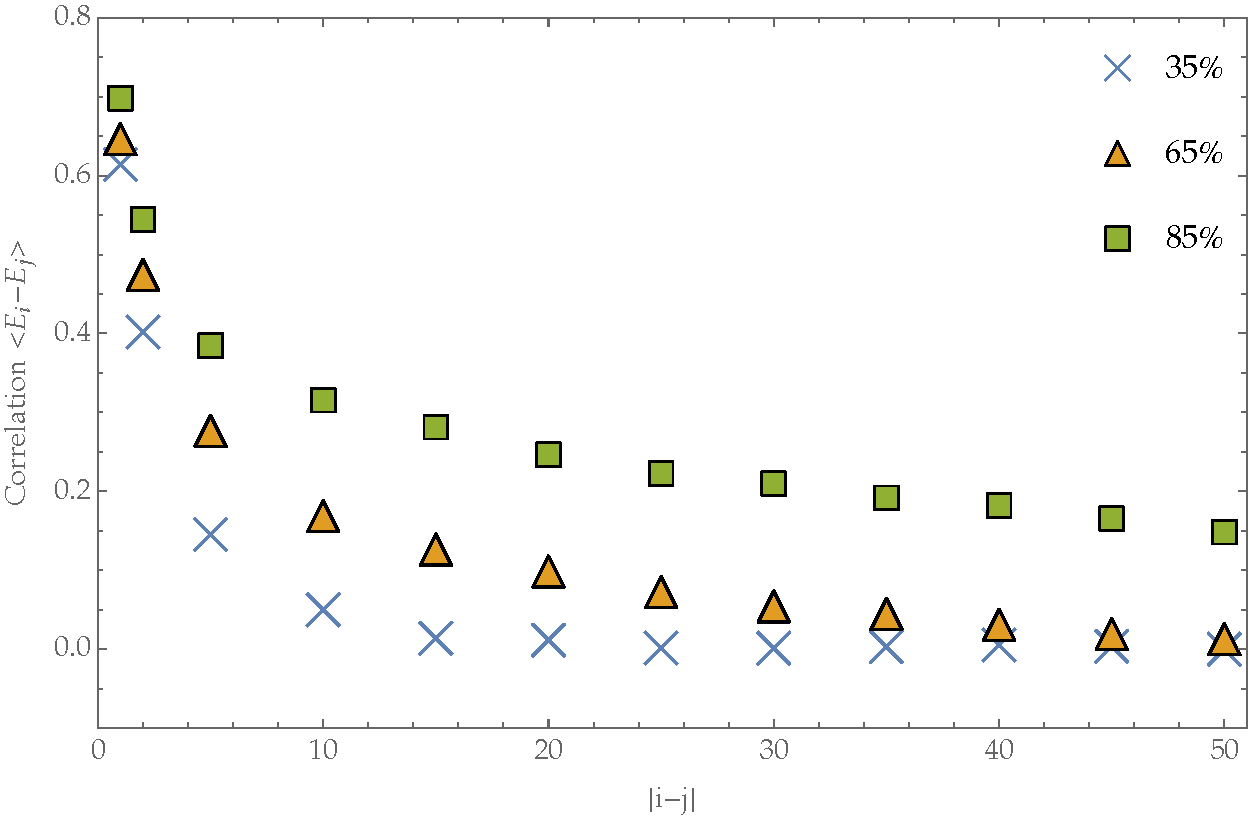
\includegraphics[width=\textwidth]{Figures/MCEnergyCorrelations.pdf}
	\caption[MC: Energy Correlation Series]{Energy correlation for a $4\times10^4$ sample. According to the acceptance ratio, the correlation length differs - also the shape of the correlation.}
	\label{fig:MCCorrSeries}
\end{figure}\\
In order to gain reasonable correlation trends, the system has to be equilibrated.
The time, until this step is reached, depends on the temperature and density of the system.
Near the critical point of the phase diagramme, the convergence behaviour is worse than apart~(see Fig.~\ref{fig:MCEnergyConvergence}).
To use nearly uncorrelated data for a meaningful quantity of interest, a smooth exponentially-decreasing correlation series and a sample distance of approximately $150$ MC-Steps has to be favored.
\begin{figure}[ht]
	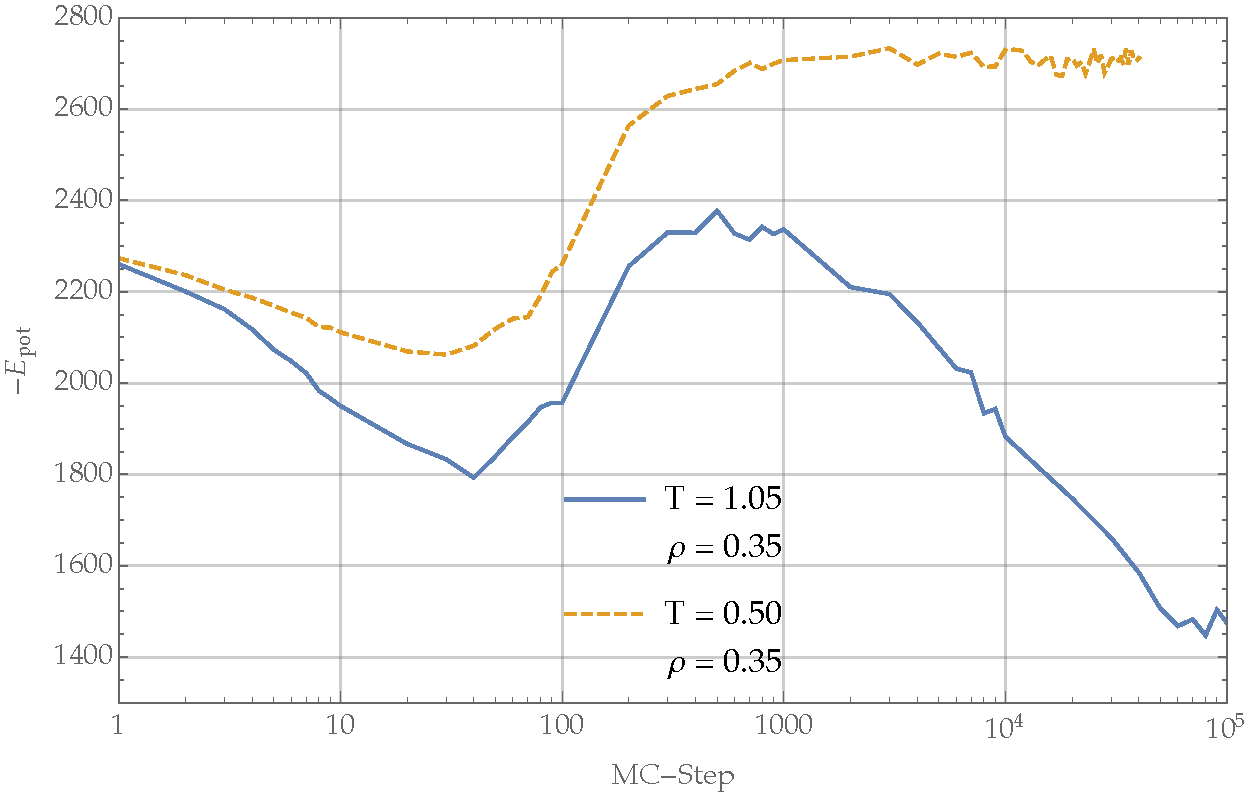
\includegraphics[width=\textwidth]{Figures/MCEnergyConvergence.pdf}
	\caption[MC: Energy Convergence Behaviour]{Energy convergence behaviour apart and near the critical point.}
	\label{fig:MCEnergyConvergence}
\end{figure}\\
In principle - one has to analyse the correlation for each measurement in particular and decide which parameters are best, but due to time frame limitations, the fixed setting is listed in Tab.~\ref{tbl:MCSettings}.
\begin{table}[ht]
	\centering
	\begin{tabular}{l | l}
		System specifics &Setting \\
		\hline
		Number of particles &chosen according to density and system size\\
		Acceptance ratio&roughly set $\approx$ \SI{60}{\percent}\\
		Equilibration&after $2\times10^6$ MC-Steps\\
		Quantity series&$6\times10^3$ samples with $150$ MC-Steps distance\\
	\end{tabular}
	\caption[MC: Settings]{Listing with settings for the measurement via Monte-Carlo.}
	\label{tbl:MCSettings}
\end{table}

\subsection{Snapshots at Different Phase Points}
The typical phase diagramme of a Lennard-Jones potential
\begin{figure}
\begin{minipage}[t]{\textwidth}
\begin{minipage}[t]{0.475\textwidth}
	\centering
	\animategraphics[width=\textwidth,autoplay,loop,controls,buttonsize=1.2em]{0.5}{/animates/MCPhase}{1}{4}
\end{minipage}
\hspace{0.5cm}
\begin{minipage}[t]{0.475\textwidth}
	\centering
	\animategraphics[width=\textwidth,autoplay,loop,controls,buttonsize=1.2em]{1}{/animates/MCPhaseSnapsT06}{0}{49}
\end{minipage}
\end{minipage}
\end{figure}
